% =====================================================================
% OPTION C — Story flowchart (top-down narrative)
% A0 vertical (841 mm × 1189 mm). Visual story: problem → idea →
% failure → fix → result, with arrows connecting boxes top to bottom.
% =====================================================================
\documentclass[a0paper, portrait]{article}

\usepackage[paperwidth=841mm, paperheight=1189mm,
            top=0mm, bottom=0mm, left=0mm, right=0mm]{geometry}
\usepackage[T1]{fontenc}
\usepackage{lmodern}
\usepackage{microtype}
\usepackage{amsmath, amssymb}
\usepackage{tikz}
\usetikzlibrary{positioning, shapes.geometric, calc, arrows.meta, fit,
                decorations.markings, backgrounds, shapes.symbols}
\usepackage{graphicx}
\usepackage{xcolor}
\usepackage{qrcode}

\pagestyle{empty}
\parindent=0pt

% --- palette ---
\definecolor{Dark}{HTML}{1A1A2E}
\definecolor{Navy}{HTML}{1F6FEB}
\definecolor{Light}{HTML}{66667A}
\definecolor{GoodGreen}{HTML}{2CA02C}
\definecolor{BadRed}{HTML}{D62C2E}
\definecolor{PaleNavy}{HTML}{F0F6FF}
\definecolor{PaleGreen}{HTML}{E8F7E8}
\definecolor{PaleRed}{HTML}{FDECEC}
\definecolor{PaleGray}{HTML}{F5F5F8}

\graphicspath{
    {../../report/figures/}
    {../../presentation/_build/}
}

% --- styles for the flow boxes ---
\tikzset{
  flow/.style={
    rectangle, rounded corners=10mm, line width=1.6mm,
    text width=620mm, inner sep=14mm,
    font=\fontsize{32}{38}\selectfont,
    align=left, anchor=north,
  },
  steparrow/.style={
    -{Latex[length=14mm, width=14mm]}, line width=3mm, color=Navy,
  },
  stepnum/.style={
    circle, fill=Navy, inner sep=0pt, minimum size=70mm,
    font=\bfseries\fontsize{56}{56}\selectfont, text=white,
  },
}

\begin{document}
\begin{tikzpicture}[remember picture, overlay,
                    every node/.style={inner sep=0pt, outer sep=0pt}]

% =====================================================================
% TITLE STRIP at top
% =====================================================================
\node[anchor=north, color=Navy,
      font=\bfseries\fontsize{28}{32}\selectfont]
    at ([yshift=-50mm]current page.north)
    {BOCCONI UNIVERSITY \;$\cdot$\; COMPUTER VISION \&\ IMAGE PROCESSING};

\node[anchor=north, color=Dark,
      font=\bfseries\fontsize{96}{106}\selectfont]
    at ([yshift=-90mm]current page.north)
    {Feedback-Augmented RT-DETR};

\node[anchor=north, color=Light,
      font=\itshape\fontsize{42}{50}\selectfont]
    at ([yshift=-180mm]current page.north)
    {The story of a silent mechanism, made measurable.};

\node[anchor=north, color=Dark,
      font=\fontsize{32}{38}\selectfont]
    at ([yshift=-235mm]current page.north)
    {Hatem Saadallah \;$\cdot$\; Nour Jennane};

% horizontal divider
\draw[Navy, line width=1.2mm]
    ([shift={(60mm,-265mm)}]current page.north west) --
    ([shift={(-60mm,-265mm)}]current page.north east);

% =====================================================================
% STEP 1 — The problem
% =====================================================================
\node[stepnum, anchor=center]
    at ([shift={(70mm,-310mm)}]current page.north west) (n1) {1};

\node[flow, draw=Navy, fill=PaleNavy]
    at ([yshift=-295mm]current page.north) (b1)
    {\textbf{\fontsize{40}{46}\selectfont\color{Navy}Small objects are hard.}\\[4mm]
     RT-DETR-R50 reports \textbf{AP\textsubscript{S}\,=\,34.7} on
     COCO val2017 --- {\itshape thirty-three points} below
     \textbf{AP\textsubscript{L}\,=\,67.7} on the same network.\\[4mm]
     \emph{Why?} Encoder memory is computed once. The decoder cannot
     revise it.};

% =====================================================================
% STEP 2 — The idea
% =====================================================================
\node[stepnum, anchor=center]
    at ([shift={(70mm,-470mm)}]current page.north west) (n2) {2};

\node[flow, draw=Navy, fill=PaleNavy]
    at ([yshift=-455mm]current page.north) (b2)
    {\textbf{\fontsize{40}{46}\selectfont\color{Navy}Let the decoder feed back.}\\[4mm]
     After layer 1 makes preliminary predictions, refine the encoder
     memory with cross-attention:
     \par\vspace{6mm}
     \centerline{$\displaystyle
        \mathbf{m}' \;=\; \mathbf{m} \;+\; g \cdot
        \mathrm{Attn}(\mathbf{m},\, \mathbf{t}^{(1)})
     $}
     \par\vspace{5mm}
     Layers 2..L then read the refined memory. \;
     $g \in (0, 1)$ is a learnable scalar gate.};

% =====================================================================
% STEP 3 — v1 failure
% =====================================================================
\node[stepnum, fill=BadRed, anchor=center]
    at ([shift={(70mm,-635mm)}]current page.north west) (n3) {3};

\node[flow, draw=BadRed, fill=PaleRed]
    at ([yshift=-620mm]current page.north) (b3)
    {\textbf{\fontsize{40}{46}\selectfont\color{BadRed}v1 trained --- and contributed nothing.}\\[4mm]
     Plain sigmoid gate, all four pyramid levels. Same-checkpoint
     ablation:\\[3mm]
     {\centering\fontsize{96}{96}\selectfont\bfseries\color{BadRed}
     $\Delta$AP\textsubscript{S}\,=\,0.00\par}
     \vspace{2mm}
     The gate decayed to ${\approx}\,0.12$. The cross-attention output
     was multiplied by zero before reaching memory.};

% =====================================================================
% STEP 4 — The fix
% =====================================================================
\node[stepnum, fill=GoodGreen, anchor=center]
    at ([shift={(70mm,-805mm)}]current page.north west) (n4) {4};

\node[flow, draw=GoodGreen, fill=PaleGreen]
    at ([yshift=-790mm]current page.north) (b4)
    {\textbf{\fontsize{40}{46}\selectfont\color{GoodGreen}Two structural fixes.
        Zero new parameters.}\\[4mm]
     \textbf{(i) Gate floor.} \;
     $g_{\mathrm{eff}} = 0.1 + 0.9\,\sigma(\alpha)$ \;
     {\itshape --- the optimizer can attenuate, never silence.}\\[5mm]
     \textbf{(ii) Level mask: P2/P3 only.} \;
     Refine stride-4 and stride-8 features (where small objects live);
     skip P4, P5.};

% =====================================================================
% Arrows between flow boxes
% =====================================================================
\foreach \from/\to in {b1/b2, b2/b3, b3/b4} {
    \draw[steparrow] (\from.south) -- ([yshift=10mm]\to.north);
}

% =====================================================================
% RESULT BANNER — the payoff
% =====================================================================
\node[fill=GoodGreen, draw=Dark, line width=2mm,
      minimum width=720mm, minimum height=110mm,
      rounded corners=12mm,
      anchor=north]
    at ([yshift=-940mm]current page.north) (rb)
    {\begin{minipage}{660mm}\centering
        {\color{white!95}\fontsize{30}{36}\selectfont
        Same-checkpoint inference ablation:}\par\vspace{1mm}
        {\color{white}\bfseries\fontsize{120}{120}\selectfont
        $\Delta$AP\textsubscript{S}\,=\,+0.99}\par\vspace{0mm}
        {\color{white!90}\itshape\fontsize{26}{32}\selectfont
        33.26 \,$\to$\, 34.25, only inference behavior changed}
     \end{minipage}};

% arrow from box 4 down to result
\draw[steparrow, color=GoodGreen, line width=4mm]
    (b4.south) -- ([yshift=10mm]rb.north);

% =====================================================================
% SUPPORTING DATA — bottom row of mini-charts (only 2 to fit)
% =====================================================================
\node[anchor=north, fill=white, draw=Light, line width=0.8mm,
      rounded corners=6mm, inner sep=6mm]
    at ([shift={(-180mm,-1075mm)}]current page.north) (chart1)
    {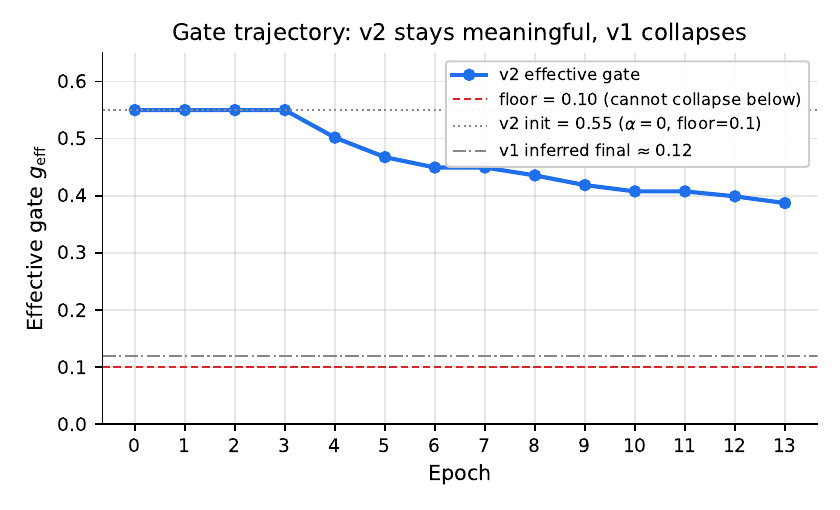
\includegraphics[width=170mm]{gate_evolution.png}};

\node[anchor=north, fill=white, draw=Light, line width=0.8mm,
      rounded corners=6mm, inner sep=6mm]
    at ([shift={(180mm,-1075mm)}]current page.north) (chart2)
    {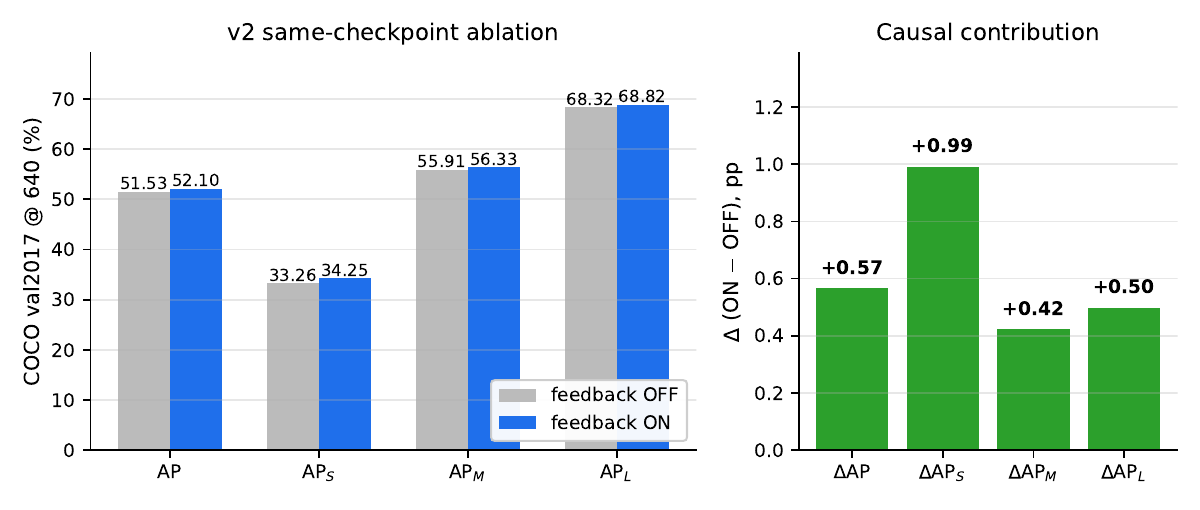
\includegraphics[width=170mm]{ablation_bars.png}};

% =====================================================================
% FOOTER
% =====================================================================
\fill[Dark]
    ([yshift=80mm]current page.south west)
    rectangle ([yshift=0mm]current page.south east);

\node[anchor=center, white,
      font=\bfseries\fontsize{30}{36}\selectfont]
    at ([yshift=55mm]current page.south)
    {Hatem Saadallah \;$\cdot$\; Nour Jennane \;$\cdot$\; Bocconi University};

\node[anchor=center, white!75,
      font=\fontsize{24}{30}\selectfont\ttfamily]
    at ([yshift=20mm]current page.south)
    {github.com/HatemSaadallah/feedback-augmented-rtdetr};

\node[anchor=south east, fill=white, inner sep=3mm]
    at ([shift={(-40mm,12mm)}]current page.south east)
    {\qrset{height=6cm}\qrcode{https://github.com/HatemSaadallah/feedback-augmented-rtdetr}};

\end{tikzpicture}
\end{document}
